Using the whisker array, we generated a dataset of whisker responses to a variety of objects.   

\textbf{Sweep Configuration.}  The dataset consists of series of simulated sweeps, mimicking one action in which the rat runs its whiskers past an object while holding its whiskers fixed (no active whisking).   
During each sweep, a single 3D object moves through the whisker array from front to back (rostral to caudal) at a constant speed.  
Each sweep lasts a total of one second, and data is sampled at 110Hz. 
Sweep scenarios vary both in terms of the identity of the object presented, as well as the position, angle, scale (defined as the length of longest axis), and speed at which it is presented.   
To simulate observed rat whisking behavior in which animals often sample an object at several vertical locations (head pitches)~\cite{hobbs2015spatiotemporal}, sweeps are performed at three different heights along the vertical axis and at each of four positions around the object (0$^{\circ}$, 90$^{\circ}$, 180$^{\circ}$, and 270$^{\circ}$ around the vertical axis), for a total of 12 sweeps per object/latent variable setting (Fig. \ref{fig_whiskers}c). 

Latent variables settings are sampled randomly and independently on each group of sweeps, with object rotation sampled uniformly within the space of all 3D rotations, object scale sampled uniformly between 25-135mm, and sweep speed sampled randomly between 77-154mm/s.  
Once these variables are chosen, the object is placed at a position that is chosen uniformly in a  $20 \times 8 \times 20$mm$^{3}$ volume centered in front of the whisker array at the chosen vertical height, and is moved along the ray toward the center of the whisker array at the chosen speed. 
The position of the object may be adjusted to avoid collisions with the fixed whisker base ellipsoid during the sweep. See implementary information for details.

The data collected during a sweep includes, for each whisker, the forces and torques from all springs connecting to the three cuboids most proximate to the base of the whisker.  This choice reflects the idea that mechanoreceptors are distributed along the entire length of the follicle at the whisker base~\cite{ebara2002similarities}.  
The collected data comprises a matrix of shape $110 \times 31 \times 3 \times 2 \times 3$, with dimensions respectively corresponding to: the 110 time samples;  the 31 spatially distinct whiskers; the 3 recorded cuboids; the forces and torques from each cuboid; and the three directional components of force/torque.   

\textbf{Object Set.} The objects used in each sweep are chosen from a subset of the ShapeNet~\cite{Chang2015} dataset, which contains over 50,000 3D objects, each with a distinct geometry, belonging to 55 categories.
Because the 55 ShapeNet categories are at a variety of levels of within-category semantic similarity, we refined the original 55 categories into a taxonomy of 117 (sub)categories that we felt had a more uniform amount of within-category shape similarity. 
The distribution of number of ShapeNet objects is highly non-uniform across categories, so we randomly subsampled objects from large categories.  
This procedure ensured that all categories contained approximately the same number of objects.  
Our final object set included 9,981 objects in 117 categories, ranging between 41 and 91 object exemplars per category (mean=85.3, median=91, std=10.2, see supplementary material for more details). 
To create the final dataset, for every object, 26 independent samples of rotation, scaling, and speed were drawn and the corresponding group of 12 sweeps created.   
Out of these 26 sweep groups, 24 were added to a training subset, while the remainder were reserved for testing.

\begin{figure}
\FigCenter
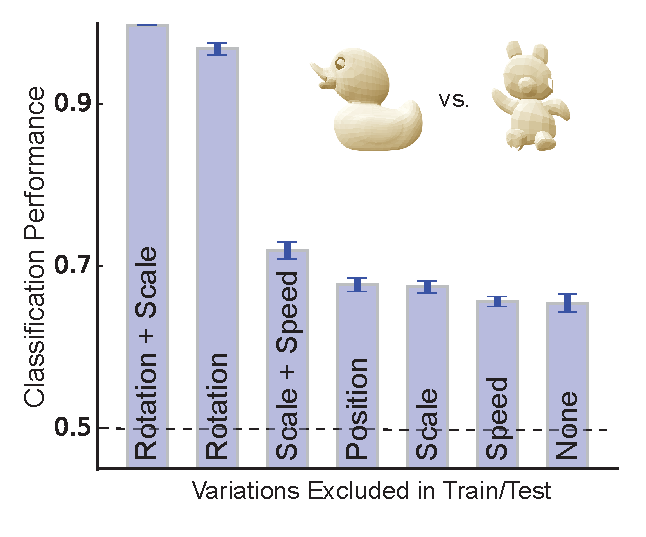
\includegraphics [width=\SmallFigSize\linewidth]{figures/control_exp.pdf}
\vspace{-3mm}
\caption{\footnotesize{\textbf{Basic validating experiment:} 
Basic validation of performance of binary linear classifier trained on raw sensor output to distinguish between two shapes (in this case, a duck versus a teddy bear).  The classifier was trained/tested on several equal-sized datasets in which variation on one or more latent variable axes is been suppressed. ``None'' indicates that all variations are present.  Dotted line represents chance performance (50\%).}~\label{fig_control}}
\vspace{-6mm}
\end{figure}

\textbf{Basic Sensor Validation.} To confirm that the whisker array was minimally functional before proceeding to more complex models, we produced smaller versions of our dataset in which sweeps were sampled densely for two objects (a bear and a duck).  
We also produced multiple easier versions of this dataset in which variation along one or several latent variables was suppressed. 
We then trained binary support vector machine (SVM) classifiers to report object identity in these datasets, using only the raw sensor data as input, and testing classification accuracy on held-out sweeps (Fig. \ref{fig_control}).  We found that with scale and object rotation variability suppressed (but with speed and position variability retained), the sensor was able to nearly perfectly identify the objects.  
However, with all sources of variability present, the SVM was just above chance in its performance,  
while combinations of variability are more challenging for the sensor than others (details can be found in supplementary information). 
Thus, we concluded that our virtual whisker array was basically functional, but that unprocessed sensor data cannot be used to directly read out object shape in anything but the most highly controlled circumstances.
As in the case of vision, it is exactly this circumstance that calls for a deep cascade of sensory processing stages. 

